\documentclass{beamer}
\setbeamertemplate{navigation symbols}{}

\setbeamercolor{frametitle}{fg=black,bg=white}
\setbeamercolor{title}{fg=black,bg=yellow!85!orange}
\usetheme{AnnArbor}

\beamersetuncovermixins{\opaqueness<1>{25}}{\opaqueness<2->{15}}
\begin{document}
\title{Clustering Overview}
\author{FRI}
\date{\today} 

\begin{frame}
\titlepage
\end{frame}

\begin{frame}
\frametitle{Applications of Clustering}
    \begin{columns}[t]
        \begin{column}[T]{9cm}
        \begin{itemize}
        \item YCbCr image compression
        \item Reading digits from images (Google)
        \end{itemize}

        \vspace{10mm}
        \hspace{7mm}
        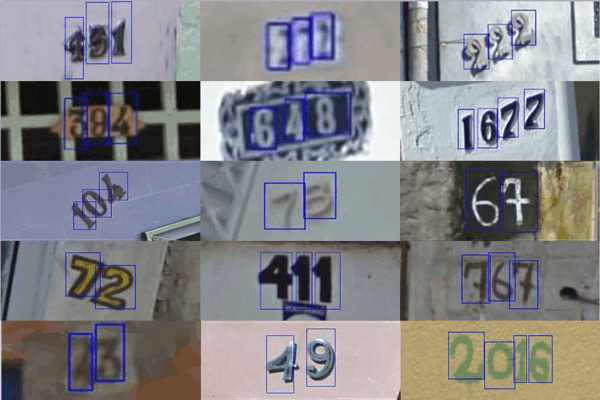
\includegraphics[height=4cm]{googlehousenumbers.jpg}

        \end{column}

        \begin{column}[T]{10cm}
        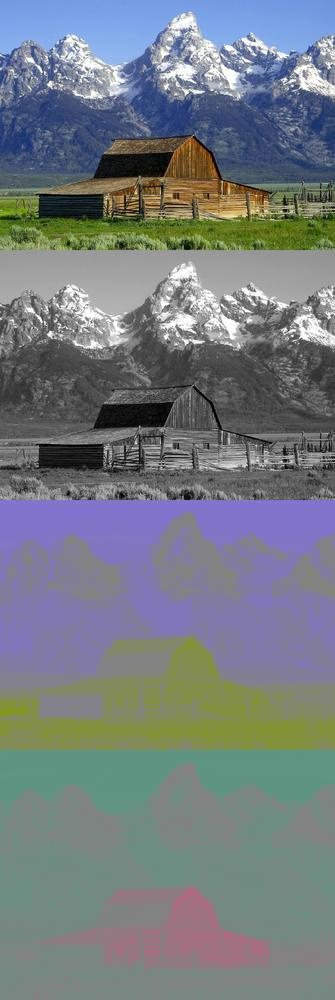
\includegraphics[height=7cm]{YCbCr-separation-small.jpg}
        \end{column}
    \end{columns}
\end{frame} 

\begin{frame}
\frametitle{YCbCr image compression}
    \begin{itemize}
    \item Human eye more sensitive to brightness than color
    \item Can reduce the bandwith of the chrominance channels
    \item Chroma subsampling
    \item NTSC, PAL, MPEG, JPEG
    \item Color quantization
    \end{itemize}
\end{frame}

\begin{frame}
\frametitle{YCbCr image compression}
    \begin{figure}[htb]
    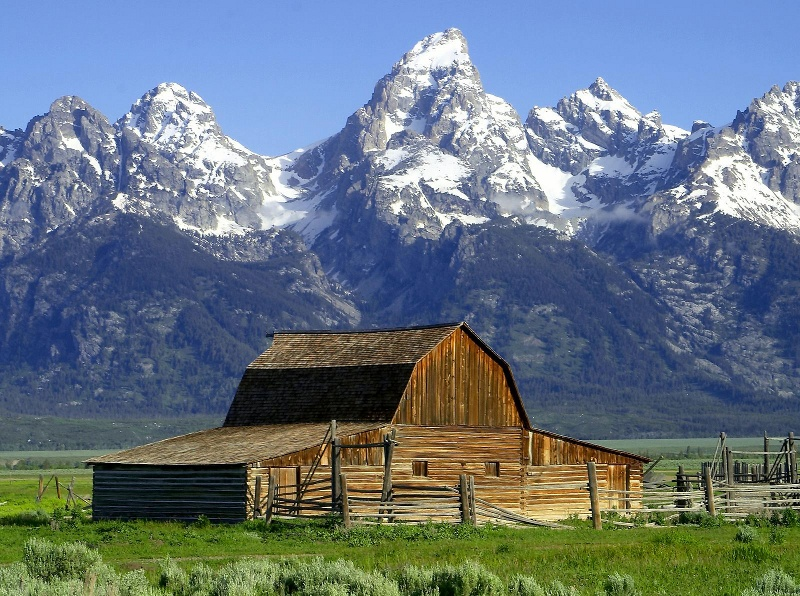
\includegraphics[scale=0.3]{YCbCr-normal.jpg}
    \end{figure}
\end{frame}

\begin{frame}
\frametitle{YCbCr image compression}
    \begin{figure}[htb]
    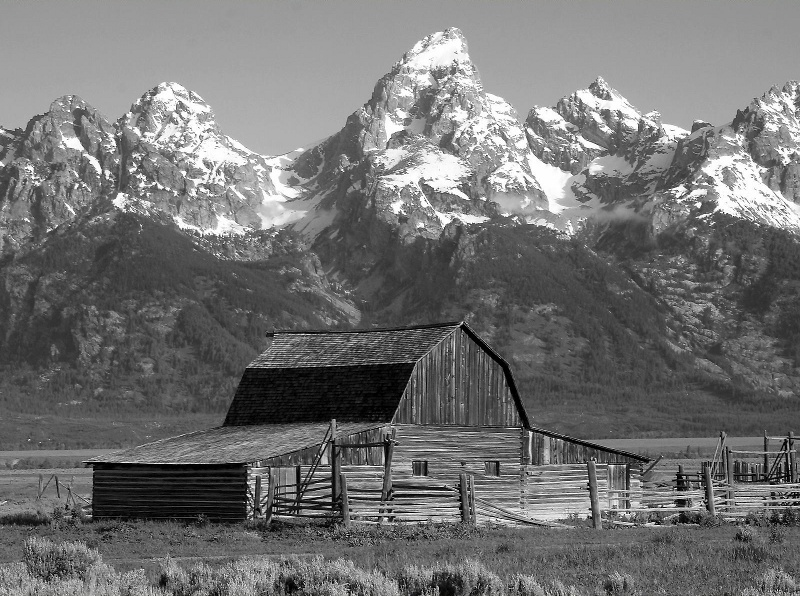
\includegraphics[scale=0.3]{YCbCr-bw.jpg}
    \end{figure}
\end{frame}

\begin{frame}
\frametitle{YCbCr image compression}
    \begin{figure}[htb]
    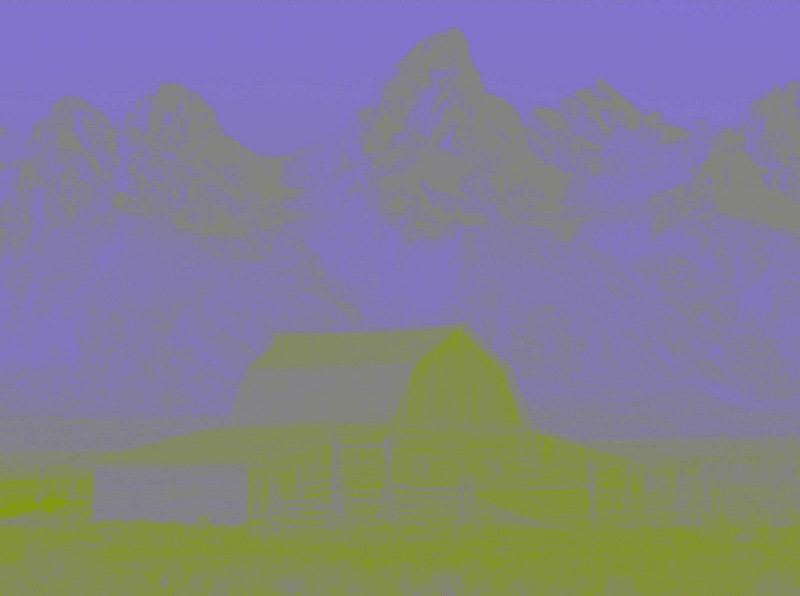
\includegraphics[scale=0.3]{YCbCr-cb.jpg}
    \end{figure}
\end{frame}

\begin{frame}
\frametitle{YCbCr image compression}
    \begin{figure}[htb]
    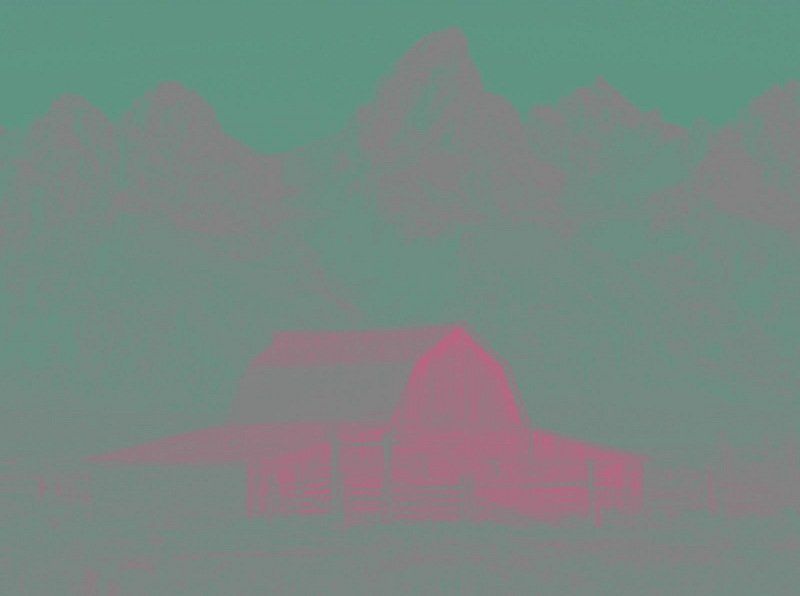
\includegraphics[scale=0.3]{YCbCr-cr.jpg}
    \end{figure}
\end{frame}

\end{document}
